% Options for packages loaded elsewhere
% Options for packages loaded elsewhere
\PassOptionsToPackage{unicode}{hyperref}
\PassOptionsToPackage{hyphens}{url}
\PassOptionsToPackage{dvipsnames,svgnames,x11names}{xcolor}
%
\documentclass[
  letterpaper,
  DIV=11,
  numbers=noendperiod]{scrartcl}
\usepackage{xcolor}
\usepackage{amsmath,amssymb}
\setcounter{secnumdepth}{5}
\usepackage{iftex}
\ifPDFTeX
  \usepackage[T1]{fontenc}
  \usepackage[utf8]{inputenc}
  \usepackage{textcomp} % provide euro and other symbols
\else % if luatex or xetex
  \usepackage{unicode-math} % this also loads fontspec
  \defaultfontfeatures{Scale=MatchLowercase}
  \defaultfontfeatures[\rmfamily]{Ligatures=TeX,Scale=1}
\fi
\usepackage{lmodern}
\ifPDFTeX\else
  % xetex/luatex font selection
\fi
% Use upquote if available, for straight quotes in verbatim environments
\IfFileExists{upquote.sty}{\usepackage{upquote}}{}
\IfFileExists{microtype.sty}{% use microtype if available
  \usepackage[]{microtype}
  \UseMicrotypeSet[protrusion]{basicmath} % disable protrusion for tt fonts
}{}
\makeatletter
\@ifundefined{KOMAClassName}{% if non-KOMA class
  \IfFileExists{parskip.sty}{%
    \usepackage{parskip}
  }{% else
    \setlength{\parindent}{0pt}
    \setlength{\parskip}{6pt plus 2pt minus 1pt}}
}{% if KOMA class
  \KOMAoptions{parskip=half}}
\makeatother
% Make \paragraph and \subparagraph free-standing
\makeatletter
\ifx\paragraph\undefined\else
  \let\oldparagraph\paragraph
  \renewcommand{\paragraph}{
    \@ifstar
      \xxxParagraphStar
      \xxxParagraphNoStar
  }
  \newcommand{\xxxParagraphStar}[1]{\oldparagraph*{#1}\mbox{}}
  \newcommand{\xxxParagraphNoStar}[1]{\oldparagraph{#1}\mbox{}}
\fi
\ifx\subparagraph\undefined\else
  \let\oldsubparagraph\subparagraph
  \renewcommand{\subparagraph}{
    \@ifstar
      \xxxSubParagraphStar
      \xxxSubParagraphNoStar
  }
  \newcommand{\xxxSubParagraphStar}[1]{\oldsubparagraph*{#1}\mbox{}}
  \newcommand{\xxxSubParagraphNoStar}[1]{\oldsubparagraph{#1}\mbox{}}
\fi
\makeatother


\usepackage{longtable,booktabs,array}
\usepackage{calc} % for calculating minipage widths
% Correct order of tables after \paragraph or \subparagraph
\usepackage{etoolbox}
\makeatletter
\patchcmd\longtable{\par}{\if@noskipsec\mbox{}\fi\par}{}{}
\makeatother
% Allow footnotes in longtable head/foot
\IfFileExists{footnotehyper.sty}{\usepackage{footnotehyper}}{\usepackage{footnote}}
\makesavenoteenv{longtable}
\usepackage{graphicx}
\makeatletter
\newsavebox\pandoc@box
\newcommand*\pandocbounded[1]{% scales image to fit in text height/width
  \sbox\pandoc@box{#1}%
  \Gscale@div\@tempa{\textheight}{\dimexpr\ht\pandoc@box+\dp\pandoc@box\relax}%
  \Gscale@div\@tempb{\linewidth}{\wd\pandoc@box}%
  \ifdim\@tempb\p@<\@tempa\p@\let\@tempa\@tempb\fi% select the smaller of both
  \ifdim\@tempa\p@<\p@\scalebox{\@tempa}{\usebox\pandoc@box}%
  \else\usebox{\pandoc@box}%
  \fi%
}
% Set default figure placement to htbp
\def\fps@figure{htbp}
\makeatother


% definitions for citeproc citations
\NewDocumentCommand\citeproctext{}{}
\NewDocumentCommand\citeproc{mm}{%
  \begingroup\def\citeproctext{#2}\cite{#1}\endgroup}
\makeatletter
 % allow citations to break across lines
 \let\@cite@ofmt\@firstofone
 % avoid brackets around text for \cite:
 \def\@biblabel#1{}
 \def\@cite#1#2{{#1\if@tempswa , #2\fi}}
\makeatother
\newlength{\cslhangindent}
\setlength{\cslhangindent}{1.5em}
\newlength{\csllabelwidth}
\setlength{\csllabelwidth}{3em}
\newenvironment{CSLReferences}[2] % #1 hanging-indent, #2 entry-spacing
 {\begin{list}{}{%
  \setlength{\itemindent}{0pt}
  \setlength{\leftmargin}{0pt}
  \setlength{\parsep}{0pt}
  % turn on hanging indent if param 1 is 1
  \ifodd #1
   \setlength{\leftmargin}{\cslhangindent}
   \setlength{\itemindent}{-1\cslhangindent}
  \fi
  % set entry spacing
  \setlength{\itemsep}{#2\baselineskip}}}
 {\end{list}}
\usepackage{calc}
\newcommand{\CSLBlock}[1]{\hfill\break\parbox[t]{\linewidth}{\strut\ignorespaces#1\strut}}
\newcommand{\CSLLeftMargin}[1]{\parbox[t]{\csllabelwidth}{\strut#1\strut}}
\newcommand{\CSLRightInline}[1]{\parbox[t]{\linewidth - \csllabelwidth}{\strut#1\strut}}
\newcommand{\CSLIndent}[1]{\hspace{\cslhangindent}#1}



\setlength{\emergencystretch}{3em} % prevent overfull lines

\providecommand{\tightlist}{%
  \setlength{\itemsep}{0pt}\setlength{\parskip}{0pt}}



 


\KOMAoption{captions}{tableheading}
\makeatletter
\@ifpackageloaded{caption}{}{\usepackage{caption}}
\AtBeginDocument{%
\ifdefined\contentsname
  \renewcommand*\contentsname{Table of contents}
\else
  \newcommand\contentsname{Table of contents}
\fi
\ifdefined\listfigurename
  \renewcommand*\listfigurename{List of Figures}
\else
  \newcommand\listfigurename{List of Figures}
\fi
\ifdefined\listtablename
  \renewcommand*\listtablename{List of Tables}
\else
  \newcommand\listtablename{List of Tables}
\fi
\ifdefined\figurename
  \renewcommand*\figurename{Figure}
\else
  \newcommand\figurename{Figure}
\fi
\ifdefined\tablename
  \renewcommand*\tablename{Table}
\else
  \newcommand\tablename{Table}
\fi
}
\@ifpackageloaded{float}{}{\usepackage{float}}
\floatstyle{ruled}
\@ifundefined{c@chapter}{\newfloat{codelisting}{h}{lop}}{\newfloat{codelisting}{h}{lop}[chapter]}
\floatname{codelisting}{Listing}
\newcommand*\listoflistings{\listof{codelisting}{List of Listings}}
\makeatother
\makeatletter
\makeatother
\makeatletter
\@ifpackageloaded{caption}{}{\usepackage{caption}}
\@ifpackageloaded{subcaption}{}{\usepackage{subcaption}}
\makeatother
\usepackage{bookmark}
\IfFileExists{xurl.sty}{\usepackage{xurl}}{} % add URL line breaks if available
\urlstyle{same}
\hypersetup{
  pdftitle={Graph Retrieval Augmented Generation and Network Analysis of the Epstein Files},
  pdfauthor={Tyler Blue; Andrew Moy; Ethan Wotring},
  colorlinks=true,
  linkcolor={blue},
  filecolor={Maroon},
  citecolor={Blue},
  urlcolor={Blue},
  pdfcreator={LaTeX via pandoc}}


\title{Graph Retrieval Augmented Generation and Network Analysis of the
Epstein Files}
\usepackage{etoolbox}
\makeatletter
\providecommand{\subtitle}[1]{% add subtitle to \maketitle
  \apptocmd{\@title}{\par {\large #1 \par}}{}{}
}
\makeatother
\subtitle{DSAN 6400 Network Analytics, Professor James Hickman}
\author{Tyler Blue \and Andrew Moy \and Ethan Wotring}
\date{2026-08-07}
\begin{document}
\maketitle

\renewcommand*\contentsname{Table of contents}
{
\hypersetup{linkcolor=}
\setcounter{tocdepth}{3}
\tableofcontents
}

\subsection*{Abstract}\label{abstract}
\addcontentsline{toc}{subsection}{Abstract}

The Epstein files have been a high profile story in the media in recent
years, and many of its documents are public data. This paper constructs
a knowledge graph connecting entities and persons in those files to
explore various techniques and metrics in the network analytics field,
such as degree, PageRank and betweenness centrality, connected component
structure, and community detection. The resulting communication network
is highly centralized. Jeffrey Epstein ranks first on every centrality
measure examined, with a weighted degree of 2,270 against 252 for the
next most active actor, and community detection within the largest
weakly connected component recovers 46 distinct communication groupings.
Furthermore, this knowledge graph is used to evaluate two retrieval
augmented generation (RAG) systems, by comparing the effectiveness of
traditional semantic search against a graph augmented RAG system. The
two systems separate along the dimension the graph was built to address.
Standard RAG scores higher on single entity lookups (7.4 against 6.8),
while GraphRAG nearly doubles its score on one hop relational questions
(6.8 against 3.6) and leads on two hop questions (5.0 against 4.0).
Ultimately, neither system dominates outright, and the graph earns its
cost precisely where semantic similarity has nothing to retrieve on,
meaning questions about how two entities are connected rather than what
a single document says.

\section{Introduction and Literature
Review}\label{introduction-and-literature-review}

Over the past several years, the collection of documents known as the
`Epstein Files' has become a widely scrutinized body of records. The
size of this collection has steadily grown through documents released in
court proceedings or released by congress, today spanning thousands of
emails and various related documents. Analysis of this large dataset is
a challenging academic task due to the scale and lack of structure of
the documents. Questions such as `who communicated with whom' and `who
was involved in this event' cannot be answered by a single document or
email, and instead require the traversal through a complicated web of
interconnected events, establishments, and people. Edge et al. (2024)
notes that queries directed at an entire corpus rather than at any
individual record are often a failure point in context retrieval
systems.

These characteristics make the Epstein Files a natural candidate for
network analysis. Rather than reading through thousands of documents to
identify structure and relationships, named entities can be extracted
from documents and linked together based on their online communications
and connections (X. Han et al. 2020). Fundamental concepts of network
analytics such as centrality and community detection can help
researchers discover influential groupings and make connections between
those involved. Organizing extracted entities and relations into a
knowledge graph is a well established way to integrate evidence spread
across heterogeneous, unstructured sources (Hogan et al. 2021).

Furthermore, by constructing a knowledge graph of the Epstein Files, a
RAG system can be augmented with additional context and information.
Typically, RAG systems rely on semantic search through vector databases
to identify relevant context to a given query (Lewis et al. 2020). This
makes it difficult to connect entities through intermediaries. For
example, two persons may be closely involved with a specific
organization, but exchange emails only with said organization, never
sharing emails between each other. A network is able to capture the
relationship between these people by identifying the organization as the
intermediary, whereas a semantic search would be completely ignorant to
it.

This paper leverages the idea of `GraphRAG' (Edge et al. 2024) to
improve the performance of a simple query based RAG system. It involves
mining contrived examples from the curated network itself to demonstrate
the inability of vector RAG to reproduce the same results, but is then
used to answer custom queries from the user via a command line
interface. Test results are scored via large language model and human
judgement. H. Han et al. (2025) show that neither system dominates
outright, with each having distinct strengths by task. Fair comparison
requires a unified protocol across both systems, which we adopt by
sharing the same model, prompt, and generation parameters.

\section{Methods}\label{methods}

\subsection{Corpus}\label{corpus}

\subsubsection{Source and Format}\label{source-and-format}

The data utilized in this project was sourced from the House Committee
on Oversight and Government Reform's 12 Nov 2025 release of 2,897
documents (U.S. House Committee on Oversight and Government Reform
2025). These documents were subpoenaed from the Department of Justice
and contain tens of thousands of pages of records, emails, and photos
from Jeffrey Epstein's estate.

The documents were obtained as an eDiscovery collection, which is a
structured collection of files typically used in the legal sector. One
distinct characteristic of this file organization is that they are
shipped with load files containing per-document metadata. They are
identified with a unique stamp and a ``Bates'' number on the first page
of each document. It was also found that page text was Optical Character
Recognition (OCR) output of scanned documents.

\subsubsection{Corpus Profiling}\label{corpus-profiling}

Due to the presence of OCR in the data aggregation, the corpus was
profiled on two independent axes. The first was ``OCR quality'', to
answer whether the characters came off the page correctly. The second
was ``Text style'', to identify whether the document has prose.

OCR quality was measured from two character level signals. The first,
the vowel-less type ratio, is the share of a document's distinct words
containing no vowels and is helpful in identifying noise in the
documents. The second, the non-word character ratio, is the share of a
document's uncommon characters, and is helpful at identifying non-prose.

Text style was measured from the common-word ratio, the share of tokens
that are common English function words. This metric identified documents
that contained running prose (ie conversations) instead of signature
blocks, financial tables, or recipient lists.

\begin{longtable}[]{@{}
  >{\raggedright\arraybackslash}p{(\linewidth - 6\tabcolsep) * \real{0.2500}}
  >{\raggedright\arraybackslash}p{(\linewidth - 6\tabcolsep) * \real{0.2500}}
  >{\raggedright\arraybackslash}p{(\linewidth - 6\tabcolsep) * \real{0.2500}}
  >{\raggedleft\arraybackslash}p{(\linewidth - 6\tabcolsep) * \real{0.2500}}@{}}
\caption{Document profiling flags (n =
2,897).}\label{tbl-profiling}\tabularnewline
\toprule\noalign{}
\begin{minipage}[b]{\linewidth}\raggedright
Axis
\end{minipage} & \begin{minipage}[b]{\linewidth}\raggedright
Flag
\end{minipage} & \begin{minipage}[b]{\linewidth}\raggedright
Meaning
\end{minipage} & \begin{minipage}[b]{\linewidth}\raggedleft
Documents
\end{minipage} \\
\midrule\noalign{}
\endfirsthead
\toprule\noalign{}
\begin{minipage}[b]{\linewidth}\raggedright
Axis
\end{minipage} & \begin{minipage}[b]{\linewidth}\raggedright
Flag
\end{minipage} & \begin{minipage}[b]{\linewidth}\raggedright
Meaning
\end{minipage} & \begin{minipage}[b]{\linewidth}\raggedleft
Documents
\end{minipage} \\
\midrule\noalign{}
\endhead
\bottomrule\noalign{}
\endlastfoot
\textbf{OCR quality} & clean & no garble signal & 2,763 (95.4\%) \\
& noisy & some garble, still readable & 100 (3.5\%) \\
& poor & heavily garbled & 33 (1.1\%) \\
& empty & effectively no text & 1 (\textless0.1\%) \\
\textbf{Text style} & prose & running text & 2,100 (72.5\%) \\
& mixed & part prose, part listing & 122 (4.2\%) \\
& sparse & few function words, such as tables, signature blocks and
lists & 49 (1.7\%) \\
& short & too few words to classify & 626 (21.6\%) \\
\end{longtable}

Documents that were flagged ``poor'' or ``empty'' were excluded from the
entity extraction, leaving 2,863 (98.8\%) of the original 2,897.

\subsubsection{Metadata Findings}\label{metadata-findings}

The finding that shaped the rest of the ingestion pipeline was that the
load file only tagged 64 documents as emails, while the OCR text
contained 4,039 email header blocks across 2,208 documents. A
communication network built from the load file fields alone would not
capture all of the correspondence that is actually present.
Figure~\ref{fig-metadata} shows the coverage of each load file field
across the release. While structural fields such as custodian and Bates
range are fully populated, the email-specific fields that a
communication network would depend on are populated for only 2\% of
documents.

\begin{figure}[H]

\centering{

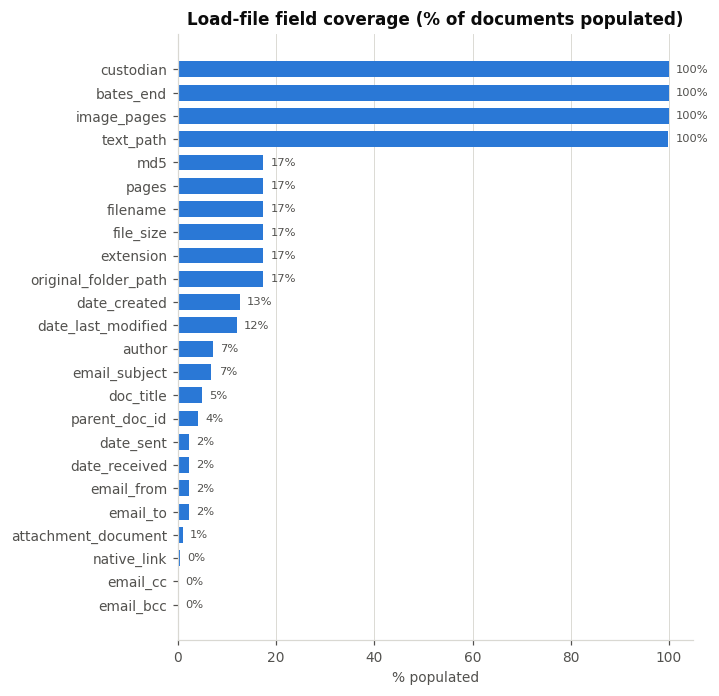
\includegraphics[width=0.85\linewidth,height=\textheight,keepaspectratio]{../results/figures/02_metadata_coverage.png}

}

\caption{\label{fig-metadata}Load-file field coverage across the
release. The email routing fields (\texttt{email\_from},
\texttt{email\_to}, \texttt{email\_cc}) are effectively empty, which is
why the communication network is reconstructed from OCR text rather than
metadata.}

\end{figure}%

\subsection{Corpus Preparation}\label{corpus-preparation}

\subsubsection{Load-file parsing and document
identity}\label{load-file-parsing-and-document-identity}

To start the corpus preparation, the metadata files of the document
release were parsed and joined to the OCR text to produce a document
manifest. This manifest is keyed on the Bates identification and
contains page ranges, per-page text offsets, and metadata fields.

\subsubsection{Text normalization with offset
preservation}\label{text-normalization-with-offset-preservation}

A large hurdle in this project was determining how to cite cleaned text,
as any transformation applied to a document will result in a citation to
the clean document, not the source. Therefore, every cleaning step was
recorded as an edit over the raw text and applied in a single pass. This
produced a table that supports direct mapping from cleaned to raw text.
As a result of this process, 97\% (3,915 of 4,050) of email edges carry
an exact page citation, greatly supporting the source document tracing
produced later in this paper.

\subsubsection{Email header parsing}\label{email-header-parsing}

Email header blocks were extracted from the normalized text using a
deterministic parser that semantically identifies the key identifiers of
email headers (``From:'', ``To:'', ``Cc:'', ``Sent:'', etc.).
Additionally, the parser splits recipient lists without breaking common
``Last, First'' display names and repairs common OCR corruption
mistakes.

Each email received a unique identification along with features such as
sender, sorted recipients, subject, and timestamp. This allowed for the
deduplication of forwarded copies of emails. As a result, 3,248 unique
messages were obtained, of which 2,704 carried both a sender and a
recipient, crucial for edge construction.

\subsection{Entity Extraction}\label{entity-extraction}

\subsubsection{Strategy and Systems}\label{strategy-and-systems}

With multiple systems available for entity extraction, the project team
found it pertinent to evaluate multiple to make an informed decision on
which to implement for the final product. Entity extraction targeted
three types, namely PERSON, Organization (ORG), and Geopolitical Entity
(GPE). The first system for entity extraction was the spaCy Python
library (Honnibal et al. 2020), specifically the
\texttt{en\_core\_web\_lg} model. The benefits of this approach were
that it only costs compute, is local, and takes about 35 minutes to run
over the corpus. The second system for entity extraction was a direct
LLM extraction using \texttt{claude-sonnet-5} across the three-type set.
While this approach is able to gather context more effectively than the
spaCy model, the cost is higher and would require a batch run for the
entire corpus. The last approach was a hybrid extraction, where an LLM
was given the text and spaCy candidates and allowed to confirm, correct,
reject, and add entities.

\subsubsection{Evaluation Design}\label{evaluation-design}

In order to evaluate the three extraction systems, 35 documents were
sampled from the corpus and stratified on OCR quality and text style
derived in the corpus profiling. Additionally, the sample was restricted
to a band of 150 to 1,500 words to limit the total number of entities
extracted. This limitation was implemented because outputs from all
three systems were pooled per document and judged at the entity level.
Two annotators determined y/n judgements of blinded, shuffled results
across 1,568 judgements.

Annotator agreement was a limitation, with Cohen's \(\kappa\) = 0.384
over 260 shared rows. The disagreement was concentrated in ORG and was
one-directional, with 48 of 56 disagreements being one annotator
accepting what the other had rejected. Per system precision differed by
10 to 17 points between annotators. As a result, absolute values should
be read as indicative, while the ranking of the systems is the true
finding of this evaluation.

\subsubsection{Results}\label{sec-extraction-results}

The evaluation of all three systems, spaCy, LLM, and hybrid can be found
in Table~\ref{tbl-extraction} and Figure~\ref{fig-extraction}. The LLM
and hybrid approaches are not distinguishable, but both outperform
spaCy. The most difficult category for all three systems was ORG, of
which no system exceeded 0.66 F1 on organizations. Consequently, this
was also the category that the annotators shared the most disagreements.

\begin{longtable}[]{@{}lrrr@{}}
\caption{Extraction system comparison. F1 is frame weighted across the
sampling strata. Corpus cost is estimated for the full 28,877 chunks via
the batch API.}\label{tbl-extraction}\tabularnewline
\toprule\noalign{}
System & F1 & ORG precision & Corpus cost \\
\midrule\noalign{}
\endfirsthead
\toprule\noalign{}
System & F1 & ORG precision & Corpus cost \\
\midrule\noalign{}
\endhead
\bottomrule\noalign{}
\endlastfoot
LLM & 0.78 & 0.79 & \textasciitilde\$64 \\
Hybrid & 0.77 & 0.75 & \textasciitilde\$64 \\
spaCy & 0.72 & 0.64 & free \\
\end{longtable}

\begin{figure}[H]

\centering{

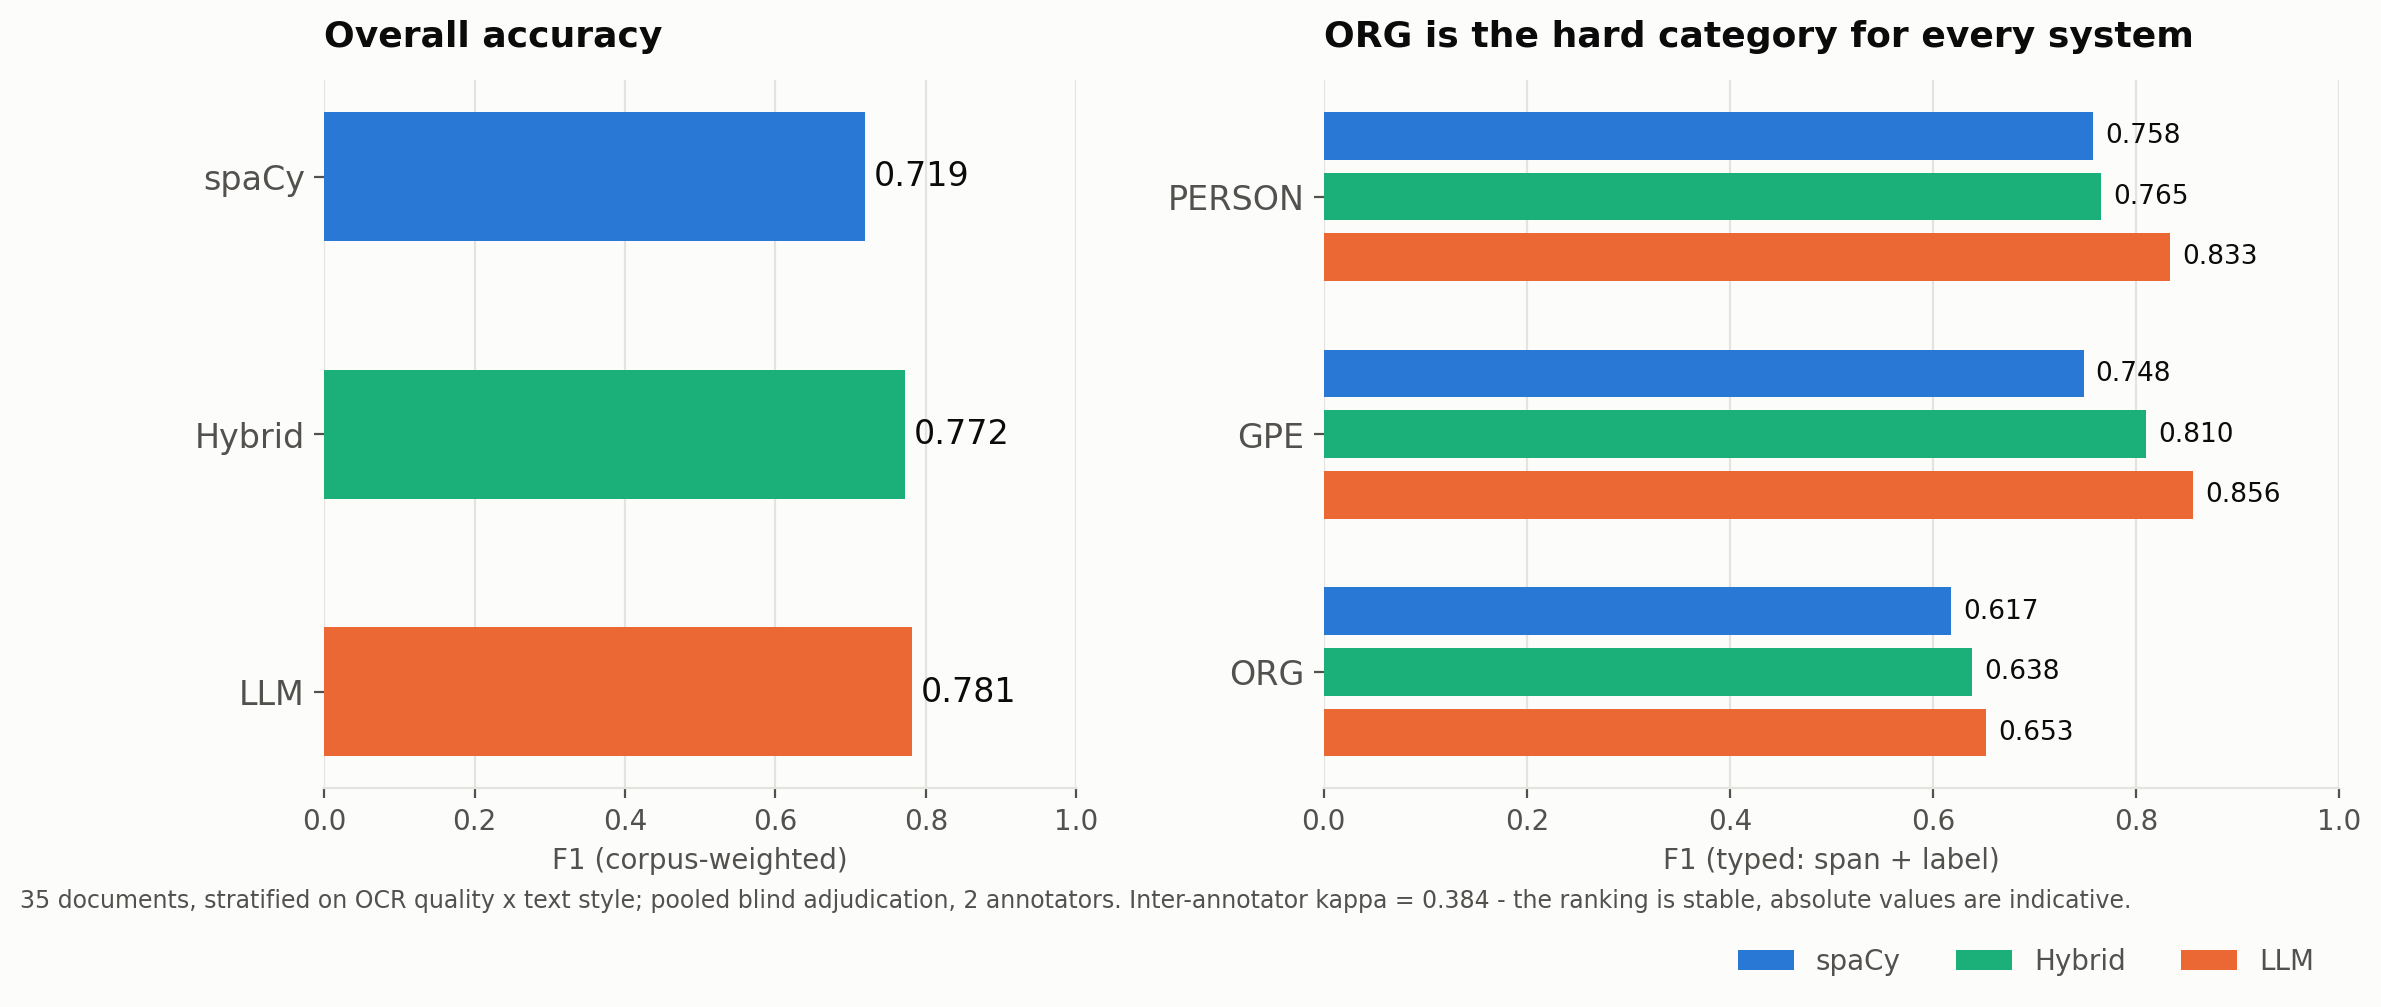
\includegraphics[width=1\linewidth,height=\textheight,keepaspectratio]{../results/figures/12_extraction_f1.png}

}

\caption{\label{fig-extraction}Extraction accuracy by system. The left
panel shows overall frame weighted F1 and the right panel shows F1 by
entity type, showing that ORG is the hardest category for every system.}

\end{figure}%

\subsubsection{Production Configuration}\label{production-configuration}

The final entity nodes are constructed with spaCy corpus wide, with
540,586 mentions over 2,857 documents resolving to 91,100 distinct
surface forms, at around 35 minutes and at no cost. LLM extraction over
the corpus was estimated at around \$64 via the batch API. The decision
to utilize spaCy over the LLM extraction was heavily weighted on the
cost and time, at the detriment of 6 F1 points of performance.

\subsection{Graph Construction}\label{graph-construction}

\subsubsection{Entity Resolution}\label{entity-resolution}

In examining the extracted entities, it was found that the number of
real entities was lacking, and significant resolution was required. For
example, one resolved entity (Jeffrey Epstein) appears as 34 different
identifiable strings. The issues in merging these aliases are twofold.
On the one hand, under-merging one person across many nodes could dilute
their centrality. On the other hand, over-merging could fabricate
relationships that propagate across the graph. Of the two, over-merging
is the more consequential.

In order to merge aliases to a single entity, comparison of extracted
entities was necessary. However, comparing all pairs resulted in 8.3
billion comparisons, which would result in countless hours of run time.
To counteract this, candidates were compared within a block depending on
the entity. For people, a block consisted of a shared surname (Epstein,
Maxwell, etc.) while organizations and places consisted of a four
character trimmed prefix.

Within a block, two names are only allowed to merge if their given names
are compatible. For example ``j epstein'' could merge with ``jeffrey
epstein'', but ``Mark Epstein'' could not. If either given name is
absent, merging is refused. Clusters are then formed by union-find, so
every merge happens without every pair being compared. Then surnames
with no given name are attached to full names using same document
evidence, with a fallback on corpus wide evidence. Additionally, email
addresses extracted from the deterministic header parser were attached
to the person whose name they match. This matching was exact or
token-order-insensitive only to preserve reliability.

As a result, 91,100 extracted strings were reduced to 81,112 entities.
It was found that only 9.3\% of entities had more than one alias, but
those entities covered 46\% of all mentions in the corpus.

\subsubsection{Edge Construction}\label{edge-construction}

Relations were built in two tiers, deterministic and statistical.
Table~\ref{tbl-tier1} shows Tier 1 relations, which were extracted
directly from the documents.

\begin{longtable}[]{@{}lrll@{}}
\caption{Tier 1 (deterministic) relations, extracted directly from
parsed email headers.}\label{tbl-tier1}\tabularnewline
\toprule\noalign{}
Relation & n & Direction & Weight \\
\midrule\noalign{}
\endfirsthead
\toprule\noalign{}
Relation & n & Direction & Weight \\
\midrule\noalign{}
\endhead
\bottomrule\noalign{}
\endlastfoot
\texttt{communicated\_with} & 1,139 & directed & distinct messages \\
\texttt{co\_recipient\_of} & 693 & undirected & messages addressed to
both \\
\texttt{participated\_in} & 1,080 & person → thread & messages
contributed \\
\end{longtable}

Email actors were mapped onto resolved entities by email address first,
then exact or token-reordered name. No fuzzy matching was used because
this is the strongest evidence of communication in the corpus and a
wrong link would fabricate a conversation. Email threads were
reconstructed by grouping messages that share a normalized subject, a
participant, and fall within 30 days. The time window of 30 days proved
necessary in thread construction, as a single participant appears in
nearly every message. Threads are modelled as nodes instead of groups of
participants to reduce inflation of every participant's centrality.
Temporal attributes were also applied to communication edges and 97\% of
email headers carried a parseable timestamp.

Tier 2 edges represent statistical associations between entities rather
than relationships explicitly stated in the source documents. An edge is
created when two entities appear together within the same text chunk,
and its strength is measured using Normalized Pointwise Mutual
Information (NPMI), which evaluates whether two entities co-occur more
frequently than would be expected based on their individual occurrence
rates. To reduce noise, entities were required to appear in at least
three chunks, while entity pairs had to co-occur in at least three
chunks across two or more documents. Additional filters removed very
large chunks, such as directories, and excluded duplicated email headers
introduced during chunking. Because NPMI can assign very high scores to
boilerplate text (e.g., email signatures or letterheads), it was used
only to identify statistically meaningful associations rather than as a
measure of relationship importance. Reported co-occurrence relationships
are instead ranked by their raw co-occurrence frequency. Every edge
retains provenance information, including the originating documents and
Bates page numbers, allowing any relationship identified by the graph or
GraphRAG system to be traced back to the original source documents. The
final network consists of 81,796 nodes and 113,613 edges, including
110,701 statistical co-occurrence edges spanning 12,864 unique entities.

\subsection{Network Analysis}\label{network-analysis}

To characterize the communication structure contained within the broader
knowledge graph, a directed communication network was constructed using
the deterministic \texttt{communicated\_with} relationships described
above. The full graph contains several types of entities and
relationships, including organizations, locations, threads,
co-occurrences, and communication events. Because the purpose of this
portion of the analysis was to evaluate communication behavior
specifically, nodes previously flagged as noisy were excluded and the
edge set was restricted to direct communication relationships. This
produced a focused communication network containing 850 nodes and 1,132
directed edges. This is slightly fewer than the 1,139
\texttt{communicated\_with} edges in Table~\ref{tbl-tier1}, because the
noise filter removed nodes along with the edges attached to them. Edge
direction represents the sender to recipient flow of communication,
while edge weight represents the number of distinct messages exchanged.

Several complementary network metrics were used to evaluate structural
importance. Degree based measures were calculated to identify highly
connected actors, with weighted degree used to capture total
communication volume. PageRank (Page et al. 1999) was calculated on the
weighted directed graph to identify actors whose importance was
reinforced through connections to other highly connected individuals.
Betweenness centrality (Freeman 1977) was calculated using network
topology to identify actors that frequently lie on shortest
communication paths and may therefore serve as brokers between otherwise
separated portions of the network.

The overall structure of the network was then evaluated using connected
component and community analysis. Weakly connected components were used
to identify portions of the graph that remain connected when edge
direction is ignored, while strongly connected components were used to
evaluate mutual reachability through directed communication paths.
Community detection was performed on the largest weakly connected
component using greedy modularity optimization (Clauset, Newman, and
Moore 2004) after converting that component to an undirected
representation. This approach identifies clusters of actors whose
communication relationships are more densely concentrated within the
group than with the remainder of the network.

Finally, both static and interactive visualizations were constructed to
support interpretation of the network. Static NetworkX (Hagberg, Schult,
and Swart 2008) visualizations used node size to represent structural
importance and node color to represent detected community membership. An
interactive PyVis visualization was also produced, allowing users to
search for actors, inspect local neighborhoods, zoom and pan through the
graph, and explore communication structure directly.

\subsection{Natural Language Querying}\label{natural-language-querying}

A major goal of this project is to build a natural language querying
system that allows a user to ask questions about the Epstein files using
natural language. To accomplish this, two approaches were used. Firstly,
a traditional RAG based pipeline was built to answer user queries about
the documents. The methodology behind the naive RAG pipeline will be
discussed first below.

\subsubsection{Vector Based RAG}\label{vector-based-rag}

The flowchart shown in Figure~\ref{fig-ragflow} below describes the
overall process for the RAG pipeline. The raw email documents will be
parsed/split into paragraph based text chunks, embedded into their
vectorized representations, and stored in a local vector database.
Queries will be submitted via command line argument, embedded into a
vector, and used to retrieve similar documents via semantic search. The
natural language query and retrieved documents will be fed into a large
language model, which will return the answer to the query.

\begin{figure}[H]

\centering{

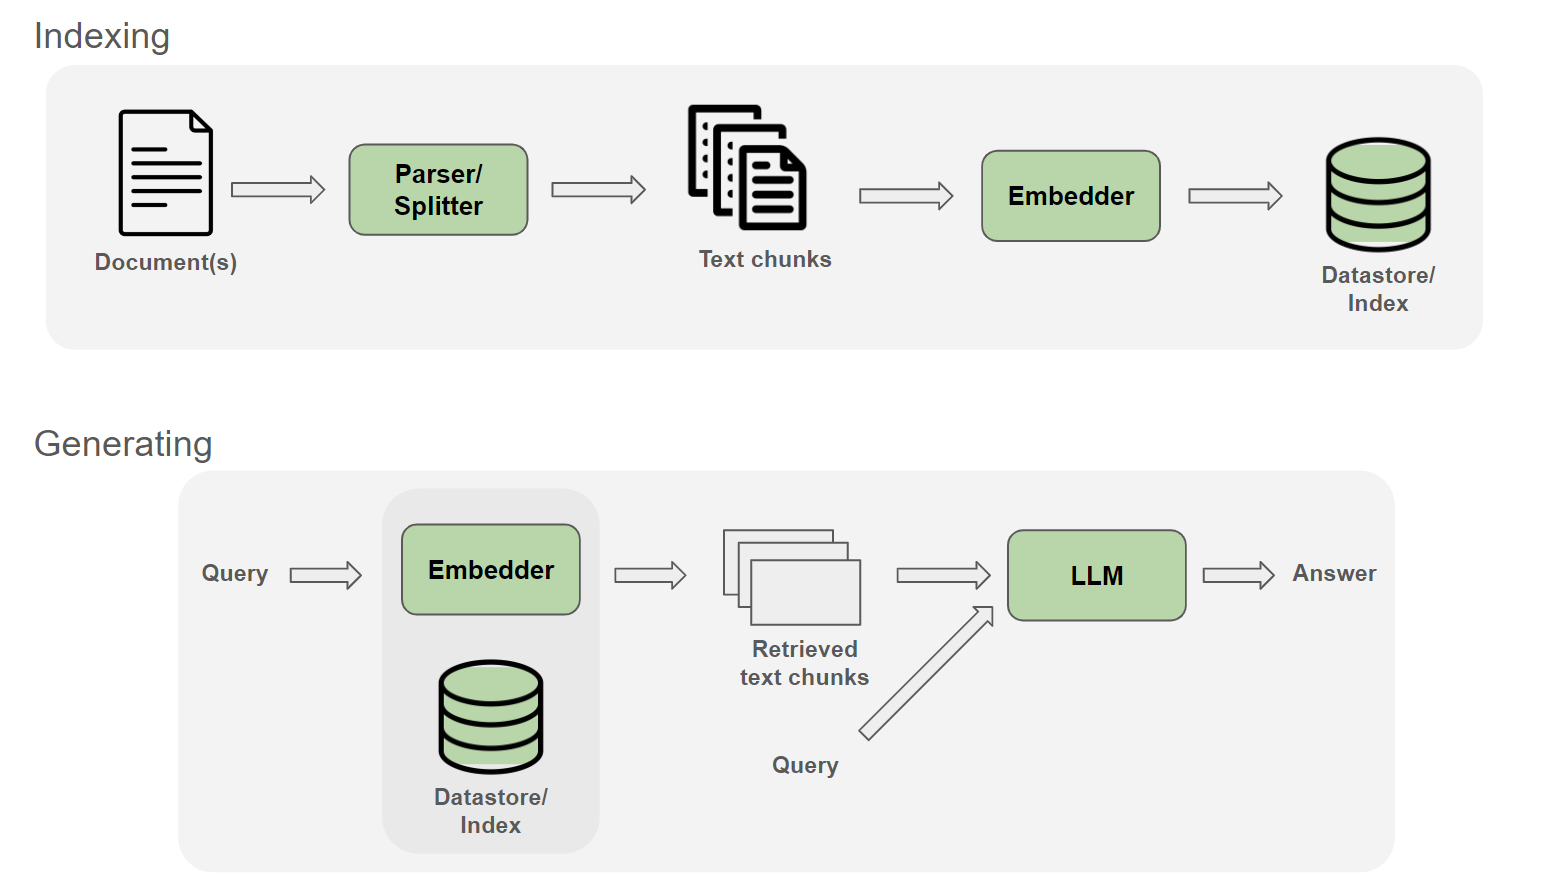
\includegraphics[width=0.95\linewidth,height=\textheight,keepaspectratio]{../results/figures/13_rag_flowchart.png}

}

\caption{\label{fig-ragflow}Flowchart for a standard RAG pipeline.
Reproduced from the NVIDIA NeMo Framework user guide (NVIDIA 2024).}

\end{figure}%

\subsubsection{Chunking}\label{chunking}

Since the majority of the raw text data is naturally subdivided into
individual `email' entities, the chunking process is designed around
that existing structure. Emails are treated as boundaries for chunking,
and chunks do not contain material across multiple emails, unless it is
an email chain (identified by subject line), in which case this boundary
is ignored. Additionally, email `headers' containing metadata such as
sender, recipient, date, etc., are parsed deterministically and
prepended to chunks derived from the email body. Emails are split by
newline into paragraphs, which are either concatenated together (for
paragraphs under 350 words) or divided (for paragraphs over 350 words).
These chunks are then embedded into a length 384 vector using the
\texttt{BAAI/bge-small-en-v1.5} model (Xiao et al. 2023), and saved to a
FAISS file (Douze et al. 2024) for later retrieval. In total, 8,497
chunks from 4,039 emails are extracted (and 28,877 total, including
non-email chunks).

\subsubsection{Retrieval}\label{retrieval}

For a given query, the same \texttt{BAAI/bge-small-en-v1.5} embedding
model is used to vectorize the query and cosine similarity is computed
against the entire vector database, returning the top \emph{k} highest
scoring chunks (\emph{k} = 8 for this paper). These natural language
chunks, in addition to the natural language query, are fed into a large
language model via API, in this case, Claude Sonnet 5.

\subsubsection{GraphRAG}\label{graphrag}

Adding the knowledge graph to the RAG system allows for information
regarding \emph{k}-hop connections to be passed to the LLM as additional
context. Given a query, entities of interest are extracted and their
respective nodes are found by key in the graph. Relevant neighbors,
edges, and associated documents must then be deterministically filtered
to aggregate information to feed to the LLM that is both properly sized
and effective. This presents a bevy of architectural decisions that must
be made, as it is a difficult task to limit a breadth-first search to a
reasonable size, as well as to identify chunks that are relevant to the
query. For this paper, entity extraction is performed on a query, and
their associated nodes are found inside the network. All paths between
nodes of interest are fed to the LLM as context, and documents
associated with the shortest path are also appended.

\subsubsection{Evaluation}\label{evaluation}

Typically, a RAG evaluation system entails both retrieval and generation
steps. The former grades whether the correct documents were identified,
while the latter grades the output of the model. For a comparison
between traditional RAG and graph RAG, generation is made the focal
point because any retrieved document that spanned a multi hop connection
would undermine the intention and effectiveness of the graph
augmentation. Therefore, metrics such as \texttt{recall@k} and Mean
Reciprocal Rank will not be reported on in this paper in favor of
judgement of the generated responses. Instead, we will focus on the
quality of LLM generated responses using both LLM-as-judge and human
evaluation.

Evaluation questions must be built somewhat artificially via mining the
documents and the preconstructed knowledge graph because connections
hidden within the Epstein Files are unknown. Questions are divided into
four categories. Firstly, single entity questions for general RAG
evaluation are judged, followed by three categories intended for
comparison between the two systems. These are single hop questions
involving entities connected by one edge, two hop questions involving
entities whose shortest path is 2, and no path questions, whose nodes
are far apart from each other. These questions are then fed through both
the traditional RAG pipeline and the graph RAG pipeline, and their
answers are compared.

\section{Results}\label{results}

\subsection{Network Analysis}\label{network-analysis-1}

The resulting communication network is highly centralized. Jeffrey
Epstein ranked first across each of the principal centrality measures
examined. His weighted degree was 2,270, substantially greater than the
next highest value of 252 for Reid Weingarten. Epstein also received the
highest PageRank score (0.2604), followed by Reid Weingarten (0.0339)
and Michael Wolff (0.0152). This consistency across activity and
influence based measures indicates that Epstein is not only the highest
volume communicator in the network, but also occupies its dominant
structural position. Figure~\ref{fig-network} makes this structure
visible, showing a dense central core surrounded by peripheral actors
who connect to the rest of the network almost exclusively through it.

\begin{figure}[H]

\centering{

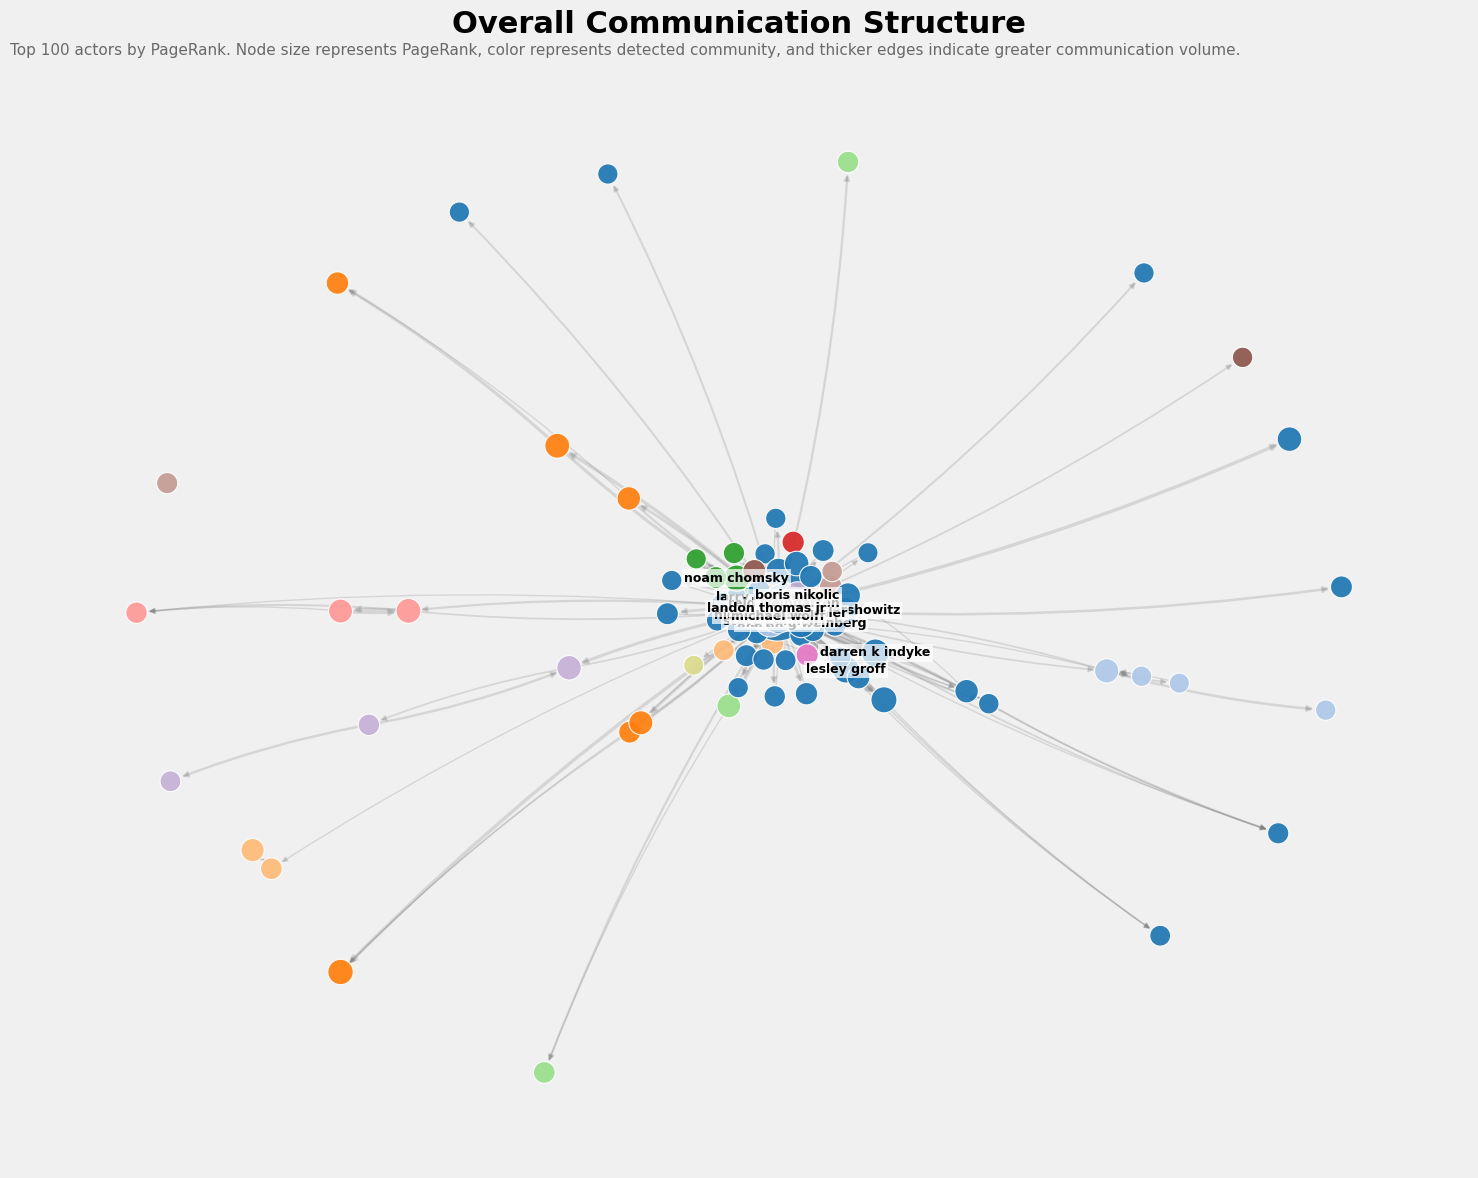
\includegraphics[width=1\linewidth,height=\textheight,keepaspectratio]{../results/figures/14_network_5.png}

}

\caption{\label{fig-network}Overall communication structure, top 100
actors by PageRank. Node size represents PageRank, color represents
detected community, and thicker edges indicate greater communication
volume.}

\end{figure}%

Betweenness centrality produced a somewhat different ranking after the
leading node, illustrating the complementary nature of the metric.
Epstein again ranked first with a betweenness score of 0.1769, while
Martin G. Weinberg ranked second at 0.0083. Other actors with relatively
high betweenness included Lesley Groff, Lawrence Krauss, Jay Lefkowitz,
and Darren K. Indyke. These individuals do not necessarily have the
largest communication volumes, but their network positions place them on
communication paths connecting otherwise more separated regions of the
graph. This distinction demonstrates why multiple centrality measures
are necessary when evaluating influence. High activity, structural
importance, and brokerage are related but not equivalent concepts.

Community detection within the largest weakly connected component
identified 46 communities. The largest community contains 252 nodes,
followed by communities of 72, 45, 39, and 36 nodes
(Figure~\ref{fig-communities}). The uneven distribution of community
sizes suggests that the network is composed of several major
communication environments alongside smaller, more specialized clusters.
These communities should be interpreted as structural communication
groupings rather than evidence of formal organizational membership or
coordinated behavior.

\begin{figure}[H]

\centering{

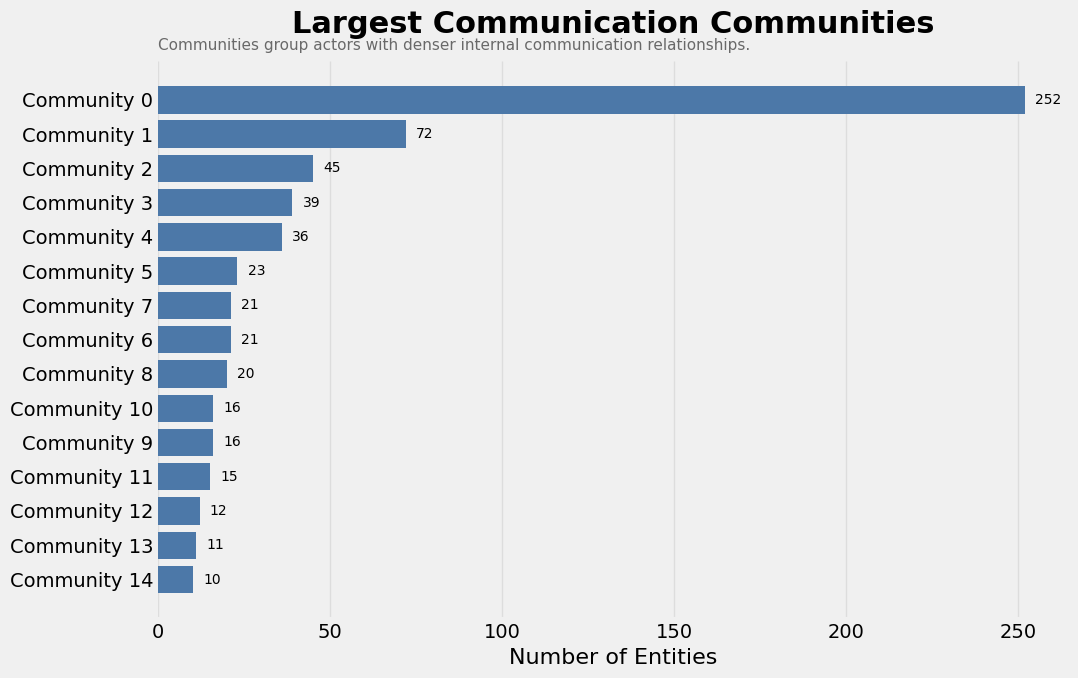
\includegraphics[width=0.85\linewidth,height=\textheight,keepaspectratio]{../results/figures/14_network_4.png}

}

\caption{\label{fig-communities}Community sizes within the largest
weakly connected component. The distribution is heavily uneven, with one
dominant community and a long tail of smaller clusters.}

\end{figure}%

Taken together, the network analysis shows that the communication graph
is dominated by a central hub but also contains meaningful internal
structure. Centrality measures identify the actors occupying the most
influential and intermediary positions, while component and community
analysis reveal how those actors are organized into broader
communication neighborhoods. These structural properties also provide a
direct bridge to the GraphRAG portion of the project. Rather than
retrieving evidence solely through semantic similarity, communities,
central actors, and graph paths can be used to guide retrieval across
related documents and entities.

\subsection{RAG vs GraphRAG}\label{rag-vs-graphrag}

Table~\ref{tbl-ragvsgraph} reports the mean judged score for each
question category under both systems. The two systems separate almost
exactly along the dimension the graph was built to address.

\begin{longtable}[]{@{}lrr@{}}
\caption{Mean judged answer quality by question category. Higher is
better. }\label{tbl-ragvsgraph}\tabularnewline
\toprule\noalign{}
Category & RAG & GraphRAG \\
\midrule\noalign{}
\endfirsthead
\toprule\noalign{}
Category & RAG & GraphRAG \\
\midrule\noalign{}
\endhead
\bottomrule\noalign{}
\endlastfoot
Single Entity & \textbf{7.4} & 6.8 \\
One Hop & 3.6 & \textbf{6.8} \\
Two Hop & 4.0 & \textbf{5.0} \\
No Path & 10.0 & 10.0 \\
\end{longtable}

On single entity questions, where the answer is contained in one
document and semantic similarity is sufficient to find it, standard RAG
scores slightly higher (7.4 against 6.8). The graph adds nothing here,
and the additional context it supplies appears to dilute rather than
sharpen the answer.

The picture reverses on relational questions. On one hop questions
GraphRAG nearly doubles the score of standard RAG (6.8 against 3.6), and
on two hop questions it retains a smaller but consistent lead (5.0
against 4.0). This is the expected result. When the answer depends on a
connection between two entities rather than the content of any single
chunk, semantic search has nothing to retrieve on, because no document
states the relationship directly. The declining margin between one hop
and two hop questions suggests that the benefit of graph augmentation
weakens as path length grows, likely because longer paths introduce more
intermediate context for a fixed context budget.

Both systems score a perfect 10.0 on no path questions. Neither
fabricated a connection between entities that are not related in the
graph, which is the correct behavior and a useful negative control. A
system that hallucinated relationships would be exposed by exactly this
category.

These results are consistent with H. Han et al. (2025), who find that
neither paradigm dominates outright across task types. The practical
implication is that the two retrieval strategies are complementary
rather than competing. A production system would route single entity
lookups to vector retrieval and relational questions to the graph.

\section{Discussion}\label{discussion}

The central finding of this project is that the structure of a document
collection determines which retrieval strategy works on it. The Epstein
Files are a correspondence corpus, and correspondence encodes
relationships that no individual document states outright. That is
precisely the case where vector retrieval fails and graph traversal
succeeds. The network analysis and the GraphRAG evaluation are two views
of the same property.

Three limitations qualify these results. First, entity extraction used
spaCy rather than the best-performing system evaluated, trading
approximately 6 F1 points for zero marginal cost. Graph derived results
should therefore be read as a lower bound on what the method can
achieve. Second, inter-annotator agreement on the extraction evaluation
was low (\(\kappa\) = 0.384), so the ranking of extraction systems is
the defensible finding while absolute scores are indicative. Third, the
evaluation question set was mined from the graph itself, which measures
whether GraphRAG can retrieve what the graph already encodes rather than
whether the graph encodes the right things.

\section{Conclusion}\label{conclusion}

This project converted 2,897 unstructured, OCR-derived documents into a
knowledge graph of 81,796 nodes and 113,613 edges, and used it for two
purposes. Network analysis showed a highly centralized communication
structure with a single dominant hub and 46 distinct communities. The
GraphRAG evaluation showed that graph augmentation nearly doubles answer
quality on one hop relational questions while offering no advantage on
single entity lookups. Neither retrieval strategy is uniformly better.
The useful result is knowing which questions belong to which.

\section*{References}\label{references}
\addcontentsline{toc}{section}{References}

\phantomsection\label{refs}
\begin{CSLReferences}{1}{0}
\bibitem[\citeproctext]{ref-clauset2004finding}
Clauset, Aaron, M. E. J. Newman, and Cristopher Moore. 2004. {``Finding
Community Structure in Very Large Networks.''} \emph{Physical Review E}
70 (6): 066111. \url{https://doi.org/10.1103/PhysRevE.70.066111}.

\bibitem[\citeproctext]{ref-douze2024faiss}
Douze, Matthijs, Alexandr Guzhva, Chengqi Deng, Jeff Johnson, Gergely
Szilvasy, Pierre-Emmanuel Mazaré, Maria Lomeli, Lucas Hosseini, and
Hervé Jégou. 2024. {``The {Faiss} Library.''}
\url{https://arxiv.org/abs/2401.08281}.

\bibitem[\citeproctext]{ref-edge2024graphrag}
Edge, Darren, Ha Trinh, Newman Cheng, Joshua Bradley, Alex Chao, Apurva
Mody, Steven Truitt, Dasha Metropolitansky, Robert Osazuwa Ness, and
Jonathan Larson. 2024. {``From Local to Global: A {GraphRAG} Approach to
Query-Focused Summarization.''} \url{https://arxiv.org/abs/2404.16130}.

\bibitem[\citeproctext]{ref-freeman1977betweenness}
Freeman, Linton C. 1977. {``A Set of Measures of Centrality Based on
Betweenness.''} \emph{Sociometry} 40 (1): 35--41.
\url{https://doi.org/10.2307/3033543}.

\bibitem[\citeproctext]{ref-hagberg2008networkx}
Hagberg, Aric A., Daniel A. Schult, and Pieter J. Swart. 2008.
{``Exploring Network Structure, Dynamics, and Function Using
{NetworkX}.''} In \emph{Proceedings of the 7th Python in Science
Conference (SciPy2008)}, 11--15.

\bibitem[\citeproctext]{ref-han2025ragvsgraphrag}
Han, Haoyu, Li Ma, Yu Wang, Harry Shomer, Yongjia Lei, Zhisheng Qi, Kai
Guo, et al. 2025. {``{RAG} Vs. {GraphRAG}: A Systematic Evaluation and
Key Insights.''} \url{https://arxiv.org/abs/2502.11371}.

\bibitem[\citeproctext]{ref-han2020relation}
Han, Xu, Tianyu Gao, Yankai Lin, Hao Peng, Yaoliang Yang, Chaojun Xiao,
Zhiyuan Liu, Peng Li, Maosong Sun, and Jie Zhou. 2020. {``More Data,
More Relations, More Context and More Openness: A Review and Outlook for
Relation Extraction.''} \url{https://arxiv.org/abs/2004.03186}.

\bibitem[\citeproctext]{ref-hogan2021knowledge}
Hogan, Aidan, Eva Blomqvist, Michael Cochez, Claudia d'Amato, Gerard de
Melo, Claudio Gutiérrez, José Emilio Labra Gayo, et al. 2021.
{``Knowledge Graphs.''} \url{https://arxiv.org/abs/2003.02320}.

\bibitem[\citeproctext]{ref-honnibal2020spacy}
Honnibal, Matthew, Ines Montani, Sofie Van Landeghem, and Adriane Boyd.
2020. {``{spaCy}: Industrial-Strength Natural Language Processing in
{Python}.''} Zenodo. \url{https://doi.org/10.5281/zenodo.1212303}.

\bibitem[\citeproctext]{ref-lewis2020rag}
Lewis, Patrick, Ethan Perez, Aleksandra Piktus, Fabio Petroni, Vladimir
Karpukhin, Naman Goyal, Heinrich Küttler, et al. 2020.
{``Retrieval-Augmented Generation for Knowledge-Intensive {NLP}
Tasks.''} In \emph{Advances in Neural Information Processing Systems}.
Vol. 33.

\bibitem[\citeproctext]{ref-nvidia2024ragoverview}
NVIDIA. 2024. {``{RAG} Overview.''} NeMo Framework User Guide.
\url{https://docs.nvidia.com/nemo-framework/user-guide/24.07/rag/ragoverview.html}.

\bibitem[\citeproctext]{ref-page1999pagerank}
Page, Lawrence, Sergey Brin, Rajeev Motwani, and Terry Winograd. 1999.
{``The {PageRank} Citation Ranking: Bringing Order to the Web.''}
1999-66. Stanford InfoLab.

\bibitem[\citeproctext]{ref-oversight2025epstein}
U.S. House Committee on Oversight and Government Reform. 2025.
{``Documents Produced by the Department of Justice Pursuant to Subpoena
(Jeffrey Epstein Estate Records).''}

\bibitem[\citeproctext]{ref-xiao2023cpack}
Xiao, Shitao, Zheng Liu, Peitian Zhang, and Niklas Muennighoff. 2023.
{``{C-Pack}: Packaged Resources to Advance General {Chinese}
Embedding.''} \url{https://arxiv.org/abs/2309.07597}.

\end{CSLReferences}




\end{document}
